
\documentclass[a4paper]{article}
\usepackage[a4paper,top=2cm,bottom=2cm,left=2cm,right=2cm,marginparwidth=2cm]{geometry}
\usepackage{lmodern}
\usepackage{listings}
\usepackage{amsmath}
\usepackage{amssymb}
\usepackage{bm}
\usepackage{textpos} % package for the positioning
\usepackage{tcolorbox}
\usepackage{pgf, tikz}
\usepackage{url}
\usetikzlibrary{arrows, automata}

\setlength{\parindent}{0em}
\setlength{\parskip}{0.3em}

\usepackage{textcomp}
\begin{document}

\lstset{language=Python,upquote=true}

\setlength{\leftskip}{20pt}
\title{Lab 3 Exercise - Optimise it!}
\author{Jonathon Hare (jsh2@ecs.soton.ac.uk)}

\maketitle

% \begin{abstract}
% \end{abstract}
% \tableofcontents

This is the exercise that you need to work through \textbf{on your own} after completing the third lab session. You'll need to write up your results/answers/findings and submit this to ECS handin as a PDF document along with the other lab exercises near the end of the module (1 pdf document per lab). 

You should use \emph{no more} than one side of A4 to cover your responses to \emph{this} exercise. This exercise is worth 5\% of your overall module grade.

\section{Exploring optimisation of analytic functions}\label{analytic}
In the lab you looked at optimising Himmelblau's Function. Now we're going to explore something even more challenging. The Rastrigin Function is a fun optimisation challenge with many local minima and a single global minima:

\begin{figure}[h!]
	\center
	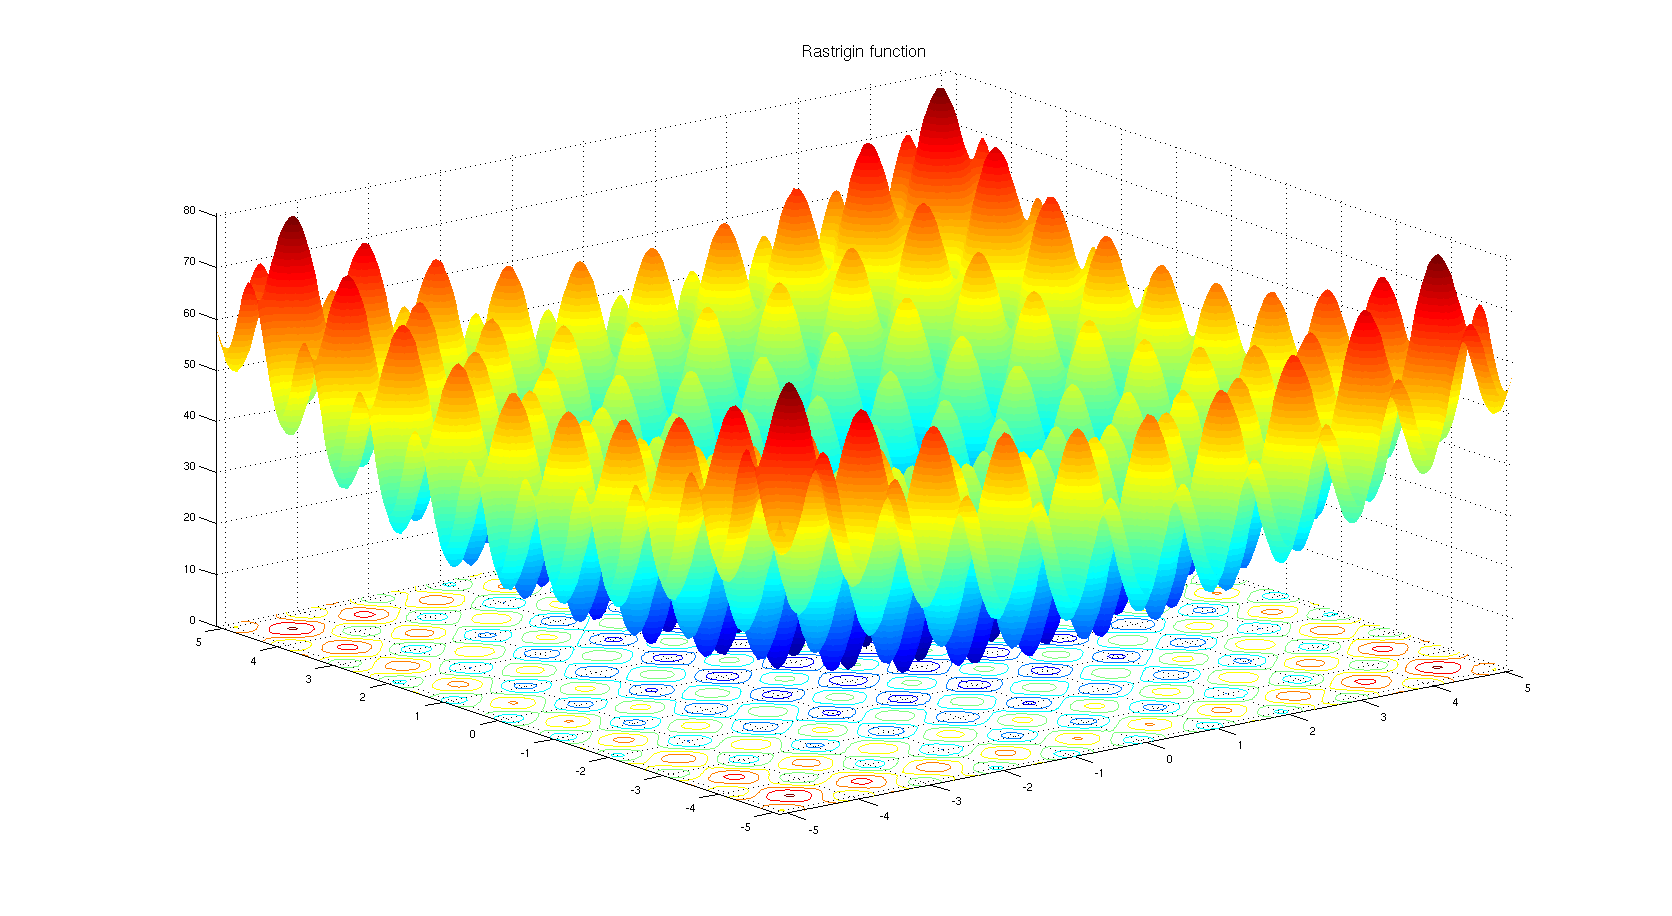
\includegraphics[width=0.8\textwidth]{Rastrigin_function.png}
\end{figure}

\begin{tcolorbox}[title=1.1 Rastrigin (3 marks)]
Consider the 2D Rastrigin function (\url{https://en.wikipedia.org/wiki/Rastrigin_function}) with $A=0.5$ (the default $A=10$ gives an extremely bumpy loss surface; smaller values are much less perturbed). Starting at $[5, 4]$ compute the point where the following optimisers arrive at after 100 iterations:

\begin{itemize}
	\item SGD (lr=0.01)
	\item SGD+Momentum (lr=0.01, momentum=0.9)
	\item Adagrad (lr=0.01)
	\item Adam (lr=0.01)
\end{itemize}

Create a loss plot showing the function value at each iteration for each of the different optimisers. Use the PyTorch implementations of the optimisers with the default values for unspecified parameters. Which optimiser works best?
\end{tcolorbox}

\section{Optimisation of a SVM on real data}\label{SVM}
The second part of the lab saw you apply a soft-margin SVM to artificially generated data and optimise its parameters with gradient descent. Now we're going to do the same with real data. Just like last week we'll use the Iris dataset, and split it into training and validation subsets (and normalise), but this time, we'll only be using two of the classes. Note that we'll also label our classes as $\{-1,1\}$:

\begin{lstlisting}[language=Python]
	import torch
	import pandas as pd
	df = pd.read_csv('https://archive.ics.uci.edu/ml/machine-learning-databases'
	  +'/iris/iris.data', header=None)
	df = df.sample(frac=1, random_state=0) #shuffle

	df = df[df[4].isin(['Iris-virginica', 'Iris-versicolor'])] #filter

	# add label indices column
	mapping = {k: v for v, k in enumerate(df[4].unique())}  
	df[5] = (2 * df[4].map(mapping)) - 1 #labels in {-1,1}

	# normalise data
	alldata = torch.tensor(df.iloc[:, [0,1,2,3]].values, dtype=torch.float)
	alldata = (alldata - alldata.mean(dim=0)) / alldata.var(dim=0)

	# create datasets
	targets_tr = torch.tensor(df.iloc[:75, 5].values, dtype=torch.long)
	targets_va = torch.tensor(df.iloc[75:, 5].values, dtype=torch.long)
	data_tr = alldata[:75]
	data_va = alldata[75:]
\end{lstlisting}

\begin{tcolorbox}[title=2.1 Iris SVM (2 marks)]
Use the following optimisers to train Soft-margin Linear SVMs (using the code from the lab notebook) with a weight decay of $0.0001$ on the training data: 
\begin{itemize}
	\item SGD (lr=0.01)
	\item SGD (lr=0.001)
	\item SGD (lr=0.0001)
	\item Adam (lr=0.01)
	\item Adam (lr=0.001)
	\item Adam (lr=0.0001)
\end{itemize}
Use a batch size of 25 and train for 100 epochs.

What is the expected validation accuracy and variance for the different models? What do you observe and why might this be the case?
\end{tcolorbox}

\end{document}



